\documentclass[a4paper,12pt]{article}
\usepackage{amsmath}
\usepackage{blindtext}
\usepackage{listings}
\usepackage[utf8]{inputenc}
\usepackage[T1]{fontenc}
\usepackage[french]{babel}
\usepackage{fullpage}
\usepackage{color}
\usepackage[table]{xcolor}
\usepackage{minibox}
\usepackage{tabularx}
\usepackage{graphicx}






\title{Projet d'Algorithmique II : Un problème de tomographie discrète}
\date{2023\\ Novembre}
\author{LU3IN003 : Groupe 3 \\ PINHO FERNANDES Enzo - 21107465 \\ DURBIN Deniz Ali - 21111116}
\newtheorem{exo}{Question}

\begin{document}
\maketitle
\tableofcontents
\newpage

\definecolor{darkWhite}{rgb}{0.94,0.94,0.94}
 
\lstset{
  aboveskip=3mm,
  belowskip=-2mm,
  backgroundcolor=\color{darkWhite},
  basicstyle=\footnotesize,
  breakatwhitespace=false,
  breaklines=true,
  captionpos=b,
  commentstyle=\color{red},
  deletekeywords={...},
  escapeinside={\%*}{*)},
  extendedchars=true,
  framexleftmargin=16pt,
  framextopmargin=3pt,
  framexbottommargin=6pt,
  frame=tb,
  keepspaces=true,
  keywordstyle=\color{blue},
  language=Python,
  literate=
  {²}{{\textsuperscript{2}}}1
  {⁴}{{\textsuperscript{4}}}1
  {⁶}{{\textsuperscript{6}}}1
  {⁸}{{\textsuperscript{8}}}1
  {€}{{\euro{}}}1
  {é}{{\'e}}1
  {è}{{\`{e}}}1
  {ê}{{\^{e}}}1
  {ë}{{\¨{e}}}1
  {É}{{\'{E}}}1
  {Ê}{{\^{E}}}1
  {û}{{\^{u}}}1
  {ù}{{\`{u}}}1
  {â}{{\^{a}}}1
  {à}{{\`{a}}}1
  {á}{{\'{a}}}1
  {ã}{{\~{a}}}1
  {Á}{{\'{A}}}1
  {Â}{{\^{A}}}1
  {Ã}{{\~{A}}}1
  {ç}{{\c{c}}}1
  {Ç}{{\c{C}}}1
  {õ}{{\~{o}}}1
  {ó}{{\'{o}}}1
  {ô}{{\^{o}}}1
  {Õ}{{\~{O}}}1
  {Ó}{{\'{O}}}1
  {Ô}{{\^{O}}}1
  {î}{{\^{i}}}1
  {Î}{{\^{I}}}1
  {í}{{\'{i}}}1
  {Í}{{\~{Í}}}1,
  morekeywords={*,...},
  numbers=left,
  numbersep=10pt,
  numberstyle=\tiny\color{black},
  rulecolor=\color{black},
  showspaces=false,
  showstringspaces=false,
  showtabs=false,
  stepnumber=1,
  stringstyle=\color{gray},
  tabsize=4,
  title=\lstname,
}

%%%%%%%%%%%%%%%%%%%%%%%%%%%%%%%%%%%%%%%%%%%%%%%%%%%%%%%%%%

\section{Méthode incomplète de résolution}

%%%%%%%%%%%%%%%%%%%%%%%%%%%%%%%%%%%%%%%%%%%%%%%%%%%%%%%%%%

\subsection{Première étape}

\begin{exo}
	Si l'on a calculé tous les $T(j,l)$, comment savoir s'il est possible de colorier la ligne $l_i$ entière avec la séquence entière ?
\end{exo}

Il est possible de colorier la ligne $l_i$ avec la séquence entière en vérifiant si $T(M-1,k)$ est défini comme vrai. En effet, ce dernier vérifie s'il est possible de colorier les $M$ premières cases de la ligne $l_i$, autrement dit toute la ligne, avec la séquence complète $(s_1,...,s_k)$.\\

\noindent\rule{\textwidth}{1pt}

%%%%%%%%%%

\begin{exo}
	Pour chacun des cas de base 1, 2a et 2b, indiquez si $T(j,l)$ prend la valeur vrai ou faux, éventuellement sous condition.
\end{exo}

Pour commencer, formulons les règles générales dans une formule. Afin que $\forall j \in {1,...,M-1}, \forall l \in {1,...,k}, T(j,l)$ soit défini comme vrai, il faut que deux conditions soient remplies.
\begin{itemize}
	\item Les $l$ premiers blocs de la séquence sont placés dans les j+1 premières cases de la ligne.
	\item Il doit y avoir exactement $l-1$ cases blanches, dans les j+1 premières cases, qui serviront de séparateur de blocs.\\
\end{itemize}

Avec cela, nous pouvons constater que cette formule doit être respectée dans n'importe quel cas : $j+1 \geq (\sum_{i=1}^{l} s_i) + l - 1$\\
Isolons $s_l$ de la somme, et $j$ du reste pour plus de maniabilité, et nous nous retrouvons avec la formule suivante :
$$j \geq (\sum_{i=1}^{l-1} s_i) + (s_l - 1) + (l-1)$$

\begin{description}
	\item[1. Cas $l=0$ (pas de bloc), $j \in \{0,...,M-1\}$] :\\ 
	Il n'y a pas de bloc à placer dans la séquence, par conséquent nous pouvons colorier toutes les cases en blanc.\\
	\minibox[frame]{$T(j,l)$ est donc vrai $\forall j \in \{0,...,M-1\}$ si $l = 0$.}

	\item[2. Cas $l \geq 0$ (au moins un bloc)] :
	\begin{description}
		\item[a. $j < s_l -1$] :\\
		Nous savons que $l \geq 1$ dans ce cas, par conséquent d'après la formule à respecter, nous aurions : $j \geq (\sum_{i=1}^{l-1} s_i) + (s_l - 1) + (l-1) \geq s_l - 1$\\
		Nous avons une contradiction, étant donné que nous sommes censés avoir : $j < s_l - 1$.\\
		\minibox[frame]{$\forall l \geq 1, T(j,l)$ est faux si $j < s_l - 1$.}

		\item[b. $j = s_l -1$] :\\ 
		Afin de répondre, nous devons séparer deux sous-cas distincts :
		\begin{itemize}
			\item \underline{Cas $l = 1$ :} $j \geq (\sum_{i=1}^{l-1} s_i) + (s_l - 1) + (l-1) = s_l - 1$\\
			Toutes les conditions sont respectées.\\
			\minibox[frame]{$T(j,l)$ est vrai si $j = s_l - 1$ et $l = 1$.}

			\item \underline{Cas $l > 1$ :} $j \geq (\sum_{i=1}^{l-1} s_i) + (s_l - 1) + (l-1) > s_l - 1$\\
			Il y a contradiction entre $j = s_l - 1$ et $j > s_l - 1$.\\
			\minibox[frame]{$T(j,l)$ est faux si $j = s_l - 1$ et $l > 1$.}
		\end{itemize}
	\end{description}
\end{description}

\noindent\rule{\textwidth}{1pt}

%%%%%%%%%%

\begin{exo}
	Exprimez une relation de récurrence permettant de calculer $T(j,l)$ dans le cas 2c en fonction de deux valeurs $T(j',l')$ avec j' $<$  j et l' $\leq$ l.
\end{exo}

Nous avons deux possibilités pour la case $(i,j)$, il suffit qu'une des deux soit vérifiée :
\begin{description}
	\item[1. La case $(i,j)$ est blanche] :\\
	La case est blanche, par conséquent il faut vérifier si nous pouvons placer le dernier bloc $s_l$ à la case précédente $j-1$, avec la même séquence. Il faut donc vérifier que $T(j-1, l)$ soit vrai.

	\item[2. La case $(i,j)$ est noire] :\\
	La case est noire, par conséquent, le bloc $s_l$ occupe les $s_l$ dernières cases. La case précédant le bloc $s_l$, si elle existe, sera coloriée en blanc. Il faut donc vérifier que $T(j-s_l-1, l-1)$ soit vrai.
\end{description}

La relation de récurrence est  donc : 
\minibox[frame]{$T(j,l) = T(j-1,l) \text{ OU } T(j-s_l-1, l-1)$}\\

\noindent\rule{\textwidth}{1pt}

%%%%%%%%%%

\begin{exo}
	Codez l'algorithme, puis testez-le.
\end{exo}

Afin d'optimiser le code, nous avons utilisé la programmation dynamique. Nous enregistrons chaque résultat d'appels récursifs dans une matrice.\\\\
Le code source est src/coloriable1.py\\

\newpage

\begin{lstlisting}
def coloriable1(j : int, l : int, s : list[int], memo : list[list[int]]) -> bool :
    """
        Renvoie vrai s'il est possible de colorier les j+1 premières cases (i,0), ..., (i,j) de la ligne l_i avec la sous-séquence (s_1, ..., s_l) des l premiers blocs de la ligne_i.
    
        Précondition : j = 0, ..., M-1 ; l = 1, ..., k; s[i] > 0 pour tout i, memo = matrice de taille M*k contenant les appels récursifs.
    """
        
    # On vérifie si on a déjà calculé T(j,l). Si c'est le cas, on renvoie directement sa valeur.
    if memo[j][l] != None :
        return memo[j][l]
    
    # Cas (1)
    elif (l == 0) :
        memo[j][l] = True
        
    # Cas (2a)
    elif (j < s[l-1] - 1) :
        memo[j][l] = False
        
    # Cas (2b)
    elif (j == s[l-1] - 1) :
        memo[j][l] = (l == 1)
    
    # Cas (2c)  
    else :
        memo[j][l] = coloriable1(j-1, l, s, memo) or coloriable1(j-s[l-1]-1, l-1, s, memo)
        
    return memo[j][l]
\end{lstlisting}

\noindent\rule{\textwidth}{1pt}
\newpage

%%%%%%%%%%

\subsection{Généralisation}

%%%%%%%%%%

\begin{exo}
	Modifiez chacun des cas de l'algorithme précédent afin qu'il prenne en compte les cases déjà coloriées.
\end{exo}

\begin{description}
	\item[1. Cas $l=0$ (pas de bloc), $j \in \{0,...,M-1\}$] :\\ 
	Ici, il n'y a pas de bloc à placer, par conséquent les $j + 1$ premières cases doivent nécessairement être blanches. Il faut donc vérifier si les $j + 1$ premières cases ne sont pas noirs. Si on en trouve au moins une, $T(j, l)$ est faux.\\
	\minibox[frame]{$T(j,l)$ est donc vrai $\forall j \in \{0,...,M-1\}$ si $l = 0$ et qu'aucune des j + 1 premières \\cases soient noires.}

	\item[2. Cas $l \geq 0$ (au moins un bloc)] :
	\begin{description}
		\item[a. $j < s_l -1$] :\\
		Dans ce cas là, d'après $(Q2)$, $T(j, l)$ est toujours faux. La couleur n'influe en rien sa valeur.
		\minibox[frame]{Pour n'importe quelle couleur, $\forall l \geq 1, T(j,l)$ est faux si $j < s_l - 1$.}

		\item[b. $j = s_l -1$] :
		\begin{itemize}
			\item \underline{Cas $l = 1$ :} Dans ce cas, les $j + 1$ premiers blocs doivent contenir le bloc $s_l$ en entier. Il faut donc vérifier si les $j + 1$ premières cases ne sont pas blanches. Si on en trouve une, $T(j, l)$ est faux.\\
			\minibox[frame]{$T(j, l)$ est vrai si $j = s_l - 1$, $l = 1$ et qu'aucune des $j+1$ premières cases\\ soient blanches.}\\

			\item \underline{Cas $l > 1$ :} Dans ce cas là, d'après $(Q2)$, $T(j, l)$ est toujours faux. La couleur n'influe en rien sa valeur.\\
			\minibox[frame]{Pour n'importe quelle couleur, $T(j,l)$ est faux si $j = s_l - 1$ et $l > 1$.}
		\end{itemize}

		\item[c. $j > s_l - 1$] :
		\begin{description}
			\item[1. La case $(i,j)$ est blanche] :\\
			La case est blanche, comme pour (Q2), il faut juste vérifier que $T(j - 1, l)$ soit vrai.
		
			\item[2. La case $(i,j)$ est noire] :\\
			La case est noire, donc il faut que le bloc $s_l$ soit placé dans les $j - sl - 1$ dernières cases, donc qu'elles ne soient pas blanches ET que la case $j - sl$ ne soit pas noire. En plus de vérifier si $T(j - sl - 1, l - 1)$ est vrai.
			Avec ces conditions, nous respectons toutes les règles du coloriage, et $T(j, l)$ sera vrai.
		\end{description}
		
	\end{description}
\end{description}

\noindent\rule{\textwidth}{1pt}
\newpage

%%%%%%%%%%

\begin{exo}
	Analysez la complexité en fonction de $M$ de l'algorithme. Pour ce faire, on déterminera le nombre de valeurs $T(j,l)$ à calculer, que l'on multipliera par la complexité de calcul de chaque valeur $T(j,l)$.
\end{exo}

\begin{itemize}
	\item Déterminons le nombre de valeurs $T(j,l)$ à calculer. Afin de stocker les résultats, nous utilisons une matrice de taille $M*k$. Maintenant, il faut essayer de borner $k$. En alternant, pour une ligne de taille $M$, chaque case en noir et blanc (cas où tous les blocs de la séquence sont de $1$ et donc que $k$ a la valeur la plus haute possible), nous pouvons constater que $k \leq \lfloor \frac{M+1}{2} \rfloor$. Nous pouvons en conclure qu'on aura un maximum de $M * \lfloor \frac{M+1}{2} \rfloor$ valeurs à calculer !

	\item Déterminons la complexité de calcul de chaque valeur $T(j,l)$. Au pire des cas, nous devons visiter un tableau contenant $M$ cases, correspond à la couleur de chaque cases $(i,j)$. On doit le parcourir entièrement, afin de vérifier s'il existe une case noire ou blanche. La complexité est donc de $\mathcal{O}(M).$
\end{itemize}

\minibox[frame]{Nous pouvons donc en conclure que la complexité de l'algorithme est de \\ $\mathcal{O}(M * (M * \lfloor \frac{M+1}{2} \rfloor)) = \mathcal{O}(M^3)$}


%%%%%%%%%%

\begin{exo}
	Codez l'algorithme.
\end{exo}

Nous avons décidé d'utiliser les entiers -1, 0, 1 afin de représenter les couleurs blanc, gris, noir respectivement.\par
Le code source est src/coloriable2.py\par

\newpage

\begin{lstlisting}
from CONSTANTES import *

def coloriable2(j : int, l : int, s : list[int], memo : list[list[int]], colors : list[int]) -> bool :
    """
        Forme améliorée de isColorable où on vérifie si une case est déjà coloriée en amont.
    
        Précondition : j = 0, ..., M-1 ; l = 1, ..., k; s[i] > 0 pour tout i, memo = matrice de taille M*k contenant les appels récursifs, colors = tableau de taille M contenant la couleur potentielle de chaque case.
    """
        
    # On vérifie si on a déjà calculé T(j,l). Si c'est le cas, on renvoie directement sa valeur.
    if memo[j][l] != None :
        return memo[j][l]
    
    # Cas (1)
    if (l == 0) :
        memo[j][l] = containsNoXColor(0, j, BLACK, colors)
        return memo[j][l]

    # Cas (2a)
    if (j < s[l-1] - 1) :
        memo[j][l] = False
        
    # Cas (2b)
    elif (j == s[l-1] - 1) :
        memo[j][l] = ((l == 1) and containsNoXColor(0, j, WHITE, colors))
    
    # Cas (2c)  
    else :
        # Cas où la case (i,j) est noire
        if colors[j] == BLACK :
            memo[j][l] = colors[j-s[l-1]] != BLACK and coloriable2(j-s[l-1]-1, l-1, s, memo, colors)  and containsNoXColor(j-s[l-1]+1, j, WHITE, colors)
            
        # Cas où la case (i,j) est blanche
        elif colors[j] == WHITE :
            memo[j][l] = coloriable2(j-1, l, s, memo, colors)
            
        # Cas où la couleur est incertaine
        else :
            whiteCase = coloriable2(j-1, l, s, memo, colors)
            if whiteCase : # Pas besoin de calculer le cas noir, on est sur un OU LOGIQUE.
                memo[j][l] = whiteCase
                return memo[j][l]
            
            memo[j][l] = colors[j-s[l-1]] != BLACK and coloriable2(j-s[l-1]-1, l-1, s, memo, colors)  and containsNoXColor(j-s[l-1]+1, j, WHITE, colors)
            
        
    return memo[j][l]



def containsNoXColor(min : int, max : int, color : int, colors : list[int]) :
    """
        Vérifie les cases (i,min), (i,min+1), ..., (i,max). Si une d'entre elle a la couleur passée en paramètre, renvoie False. Sinon True.
    """
    for i in range(min, max+1) :
        if colors[i] == color :
            return False
    return True

\end{lstlisting}

\noindent\rule{\textwidth}{1pt}
\newpage

%%%%%%%%%%

\subsection{Propagation}

\begin{exo}
	Montrez que cet algorithme est de complexité polynomiale en $N$ et $M$.
\end{exo}

\begin{itemize}
	\item Calculons la complexité de $ColoreLig()$. Cette dernière va exécuter deux fois la fonction coloriable2(), une pour tester la case blanche, l'autre pour la case noire. Il recommencera au pire des cas $M$ fois afin de parcourir toute la ligne. De plus, la complexité de coloriable2() a été calculée précédemment, nous donnant $\mathcal{O}(M^3)$. La complexité totale de $ColoreLig()$ est de $\mathcal{O}(M^4)$
	\item La même logique s'applique sur $ColoreCol()$, on aura une complexité de $\mathcal{O}(N^4)$
	\item Calculons la complexité globale. La fonction effectue une boucle tant que toutes les lignes et colonnes n'ont pas été traitées sans qu'il y ait une actualisation. Au pire cas, il y aura autant de boucle que de valeurs dans la grille, donc $M*N$. De plus, cette boucle while contient elle-même deux boucles for, tournant au maximum $N$ et $M$ fois respectivement. Et enfin, les deux boucles for appellent une fois $ColoreLig()$ et $ColoreCol()$.\\
\end{itemize}

\minibox[frame]{La complexité globale de l'algorithme est donc de $\mathcal{O}(M*N * (M*N^4 + N*M^4))$.}\\

\noindent\rule{\textwidth}{1pt}

%%%%%%%%%%

\begin{exo}
	Codez l'algorithme de propagation.
\end{exo}

\begin{description}
	\item[src/lectureInstance.py] : Permet de lire le fichier texte et de le transformer en grille, avec ses séquences.
	\item[src/Grille.py] : Classe représentant une grille. Elle possède la matrice, les variables M, N et ses séquences. De plus, elle a des fonctions afin de lire la matrice esthétiquement, ainsi que vérifier si elle est coloriée en totalité.
	\item[src/CONSTANTES.py] : Contient les constantes attribuées aux différentes couleurs, ainsi qu'une fonction pour créer facilement un mémo, pour le bien de la programmation dynamique.
	\item[src/coloreLig.py] : Teste chaque ligne pour tenter de colorier des cases en se servant de $coloriable2()$.
	\item[src/coloreCol.py] : Teste chaque colonne pour tenter de colorier des cases en se servant de $coloriable2()$.
	\item[src/coloration.py] : Colorie une grille A passé en paramètre si possible.
	\item[src/propagation.py] : Transforme le fichier texte passé en paramètre en grille, puis le résout à l'aide de $coloration()$.
	\item[src/main.py] : Teste les 16 instances fournies, et donne le temps requis pour chacune d'entre elles.
\end{description}

Attention, afin de pouvoir exécuter le main, il vaut mieux que le répertoire courant soit le $src$, afin de ne pas avoir à modifier les chemins.

\begin{center}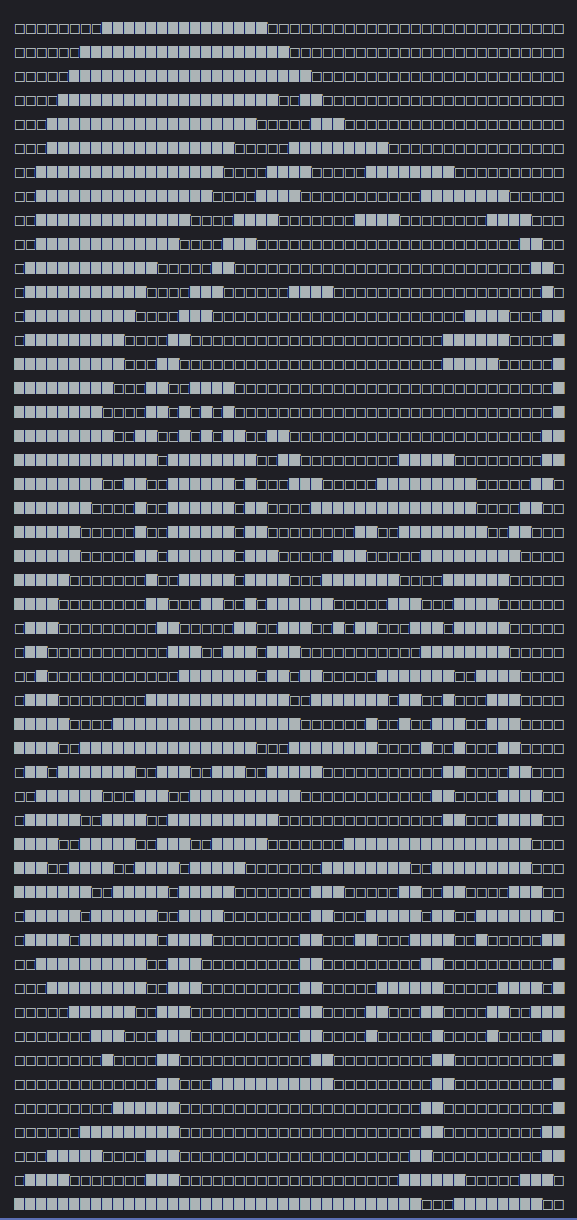
\includegraphics[width=10cm]{instance9.png}\end{center}

\newpage

\begin{table}
\centering
\begin{tabular}{|l|l|l|l|l|l|l|l|l|l|l|}
ID.Instances           & 1      & 2      & 3      & 4      & 5  \\
Temps d'exécution en s & 0.0009 & 0.0983 & 0.0685 & 0.1825 & 0.1780 
\end{tabular}
\end{table}

\begin{table}
\centering
\begin{tabular}{|l|l|l|l|l|l|l|l|l|l|l|}
ID.Instances           & 6      & 7      & 8      & 9      & 10      \\
Temps d'exécution en s &  0.3410 & 0.2420 & 0.4591 & 3.8529 & 6.4821 
\end{tabular}
\end{table}

\begin{lstlisting}

def lectureInstance(path : str) :
    """
        Lit un fichier texte dont chaque ligne correspond à la séquence associée à une ligne ou une colonne de la grille.
        Le symbole # indique que l'on passe à la description des lignes à celle des colonnes.
        Avant le #, il y a autant de lignes dans le fichier que de lignes dans la grille, et à chaque ligne est indiquée la séquence d'entiers représentant les longueurs de blocs.
        
        La fonction renvoie le grille correspondante ainsi qu'un tableau comportant les séquences lignes, et un autre tableau comportant les séquences colonnes.
    """
    # Pour commenter le code, on utilisera l'instance 0.txt comme exemple.
    
    # Lis le fichier, fileRead est un tableau de forme : ['3', '', '1 1 1', '3', '#', '1 1', '1', '1 2', '1', '2'].
    with open(path, 'r') as fp :
        fileRead : list[str] = [line.strip('\n') for line in fp.readlines()]
    
    # On trouve l'index du séparateur '#' afin de découper en deux le tableau. Un pour les séquences des lignes, et l'autre pour les séquences des colonnes.
    index_separator_lig_col : int = fileRead.index("#")
    seqs_lig : list[str] = fileRead[:index_separator_lig_col]
    seqs_col : list[str] = fileRead[index_separator_lig_col+1:]
    
    # Nous créons une liste finale comportant les séquences sous forme de liste de int.
    # On aura donc pour les lignes, [[3], [], [1, 1, 1], [3]]
    # On aura donc pour les colonnes, [[1, 1], [1], [1, 2], [1], [2]]
    seqs_lig : list[list[int]] = [list(map(int, sequence.split(' '))) if sequence else [] for sequence in seqs_lig]
    seqs_col : list[list[int]] = [list(map(int, sequence.split(' '))) if sequence else [] for sequence in seqs_col]

    # Création d'une classe Grille.   
    return Grille(seqs_lig, seqs_col)
\end{lstlisting}

\newpage

\begin{lstlisting}
class Grille :
    """
        Classe représentant une grille.
    """
    def __init__(self, sequences_lignes : list[list[int]] = [], sequences_colonnes : list[list[int]] = []) :
        self.seqs_lig = sequences_lignes
        self.seqs_col = sequences_colonnes
        
        self.N : int = len(self.seqs_lig)
        self.M : int = len(self.seqs_col)
        self.grille : list[list[int]] = [[GRAY for _ in range(self.M)] for _ in range(self.N)]
        
        
    
    def coloriageTermine(self) -> bool :
        """
            Vérifie si la grille a été entièrement colorée.
        """
        for i in range(self.N) :
            for j in range(self.M) :
                if self.grille[i][j] == GRAY :
                    return False
        return True
    
    def afficheGrille(self) -> None :
        """
            Affiche la grille en tenant compte du coloriage.
        """

        for i in range(self.N) :
            for j in range(self.M) :
                case : int = self.grille[i][j]
                if(case == BLACK) :
                    print(u"\u25A0", end = '')
                elif(case == WHITE) :
                    print(u"\u25A1", end = '')  
                else :
                    print("+", end = '')
            print()
        print()
\end{lstlisting}

\begin{lstlisting}
# CONSTANTES.PY
GRAY = 0
BLACK = 1
WHITE = 2

def creationMemo(M : int, k : int) :
    return [[None for _ in range(k + 1)] for _ in range(M)]
\end{lstlisting}

\newpage

\begin{lstlisting}
def coloreLig(A : Grille, i : int) -> (bool, Grille, set):
    ligneColors : list[int] = copy.deepcopy(A.grille[i])
    l : int = len(A.seqs_lig[i])
    Nouveaux : set = set()
    
    for z in range(A.M) :
        if (ligneColors[z]) == GRAY :
            # Test : case blanche
            memo : list[list[int]] = creationMemo(A.M, A.N)
            ligneColors[z] = WHITE
            testWhite = coloriable2(A.M - 1, l, A.seqs_lig[i], memo, ligneColors)
            
            # Test : case noire
            memo = creationMemo(A.M, A.N)
            ligneColors[z] = BLACK
            testBlack = coloriable2(A.M - 1, l, A.seqs_lig[i], memo, ligneColors)
            
            # Cas : Aucun test échoué, on ne peut rien déduire.
            if (testWhite and testBlack) :
                ligneColors[z] = GRAY
                A.grille[i][z] = GRAY
            
            # Cas : Test blanc réussi, on peut colorier la case en blanc.
            elif (testWhite and not testBlack) :
                ligneColors[z] = WHITE
                A.grille[i][z] = WHITE
                Nouveaux.add(z)
                
            # Cas : Test noir réussi, on peut colorier la case en noir.
            elif (not testWhite and testBlack) :
                ligneColors[z] = BLACK
                A.grille[i][z] = BLACK
                Nouveaux.add(z)
                
            # Cas : Aucun test réussi, le puzzle n'a pas de solution.
            else :
                return (False, A, Nouveaux)
    
    return (True, A, Nouveaux)
\end{lstlisting}

\newpage

\begin{lstlisting}
def coloreCol(A : Grille, i : int) -> (bool, Grille, set):
    colonneColors : list[int] = [ligne[i] for ligne in A.grille]
    l : int = len(A.seqs_col[i])
    Nouveaux : set = set()
    
    for z in range(A.N) :
        if colonneColors[z] == GRAY :
            # Test : case blanche
            memo : list[list[int]] = creationMemo(A.N, A.M)
            colonneColors[z] = WHITE
            testWhite = coloriable2(A.N - 1, l, A.seqs_col[i], memo, colonneColors)
            
            # Test : case noire
            memo : list[list[int]] = creationMemo(A.N, A.M)
            colonneColors[z] = BLACK
            testBlack = coloriable2(A.N - 1, l, A.seqs_col[i], memo, colonneColors)
            
            # Cas : Aucun test échoué, on ne peut rien déduire.
            if (testWhite and testBlack) :
                colonneColors[z] = GRAY
                A.grille[z][i] = GRAY
            
            # Cas : Test blanc réussi, on peut colorier la case en blanc.
            elif (testWhite and not testBlack) :
                colonneColors[z] = WHITE
                A.grille[z][i] = WHITE
                Nouveaux.add(z)
                
            # Cas : Test noir réussi, on peut colorier la case en noir.
            elif (not testWhite and testBlack) :
                colonneColors[z] = BLACK
                A.grille[z][i] = BLACK
                Nouveaux.add(z)
                
            # Cas : Aucun test réussi, le puzzle n'a pas de solution.
            else :
                return (False, A, Nouveaux)
    
    return (True, A, Nouveaux)
\end{lstlisting}

\newpage

\begin{lstlisting}
def coloration(A : Grille) :
    """
        Colore une grille A entièrement non coloriée.
    """
    
    Ap : Grille = copy.deepcopy(A)   # Pour ne pas modifier A en entrée
    LignesAVoir = [i for i in range(Ap.N)]
    ColonnesAVoir = [i for i in range(Ap.M)]
    
    while len(LignesAVoir) > 0 or len(ColonnesAVoir) > 0 :
        for i in LignesAVoir :
            ok, Ap, Nouveaux = coloreLig(Ap, i)
            if not ok :
                return (False, Grille())
            
            ColonnesAVoir = list(set(ColonnesAVoir) | Nouveaux)
            LignesAVoir.remove(i)
         
        for j in ColonnesAVoir :
            ok, Ap, Nouveaux = coloreCol(Ap, j)
            if not ok :
                return (False, Grille())
            LignesAVoir = list(set(LignesAVoir) | Nouveaux)
            ColonnesAVoir.remove(j)
        
    if Ap.coloriageTermine() :
        return (True, Ap)
    return (None, Ap)
\end{lstlisting}

\begin{lstlisting}
# main.py

from CONSTANTES import *
from propagation import *
from time import time

print("Algorithme : Méthode INCOMPLETE de résolution !")

listTempo = []
for i in range(1, 17) :
    chronoStart = time()
    propagation(f"instances/{i}.txt")
    chronoStop = time()
    listTempo.append(chronoStop - chronoStart)
    print()
    
for i in range(16) :
    print(f"Instance {i+1} : {listTempo[i]} secondes.")
\end{lstlisting}


%%%%%%%%%%%%%%%%%%%%%%%%%%%%%%%%%%%%%%%%%%%%%%%%%%%%%%%%%%

\section{Méthode complète de résolution}

%%%%%%%%%%%%%%%%%%%%%%%%%%%%%%%%%%%%%%%%%%%%%%%%%%%%%%%%%%

\begin{exo}
	Montrez que cet algorithme est de complexité exponentielle en $N$ et $M$.
\end{exo}


\end{document}